\documentclass[11pt,a4paper]{report}

\usepackage{fontspec}
\setmainfont{Arial}
\newfontfamily\arabicfont[Script=Arabic]{Arial}

\usepackage[a4paper,margin=2.5cm]{geometry}
\usepackage{xcolor}
\definecolor{esprit}{RGB}{0,70,140}
\usepackage[colorlinks=true,linkcolor=esprit,urlcolor=esprit,citecolor=esprit]{hyperref}
\usepackage{titlesec}
\usepackage{enumitem}
\usepackage{longtable}
\usepackage{booktabs}
\usepackage{fancyhdr}
\usepackage{tcolorbox}
\usepackage{tikz}
\usetikzlibrary{arrows.meta,positioning}

\titleformat{\chapter}[hang]{\normalfont\huge\bfseries\color{esprit}}{\thechapter.}{20pt}{\huge}
\titleformat{\section}{\normalfont\Large\bfseries\color{esprit}}{\thesection}{10pt}{}
\titleformat{\subsection}{\normalfont\large\bfseries}{\thesubsection}{8pt}{}

\pagestyle{fancy}
\fancyhf{}
\fancyhead[L]{ESPRIT AI Receptionist -- Rapport de projet}
\fancyhead[R]{\thepage}
\renewcommand{\headrulewidth}{0.4pt}

\newtcolorbox{statutfait}{colback=green!8,colframe=green!45!black,boxrule=0.5pt,arc=2pt,left=6pt,right=6pt,top=3pt,bottom=3pt}
\newtcolorbox{statutencours}{colback=yellow!10,colframe=orange!70!black,boxrule=0.5pt,arc=2pt,left=6pt,right=6pt,top=3pt,bottom=3pt}
\newtcolorbox{statutlimite}{colback=red!6,colframe=red!50!black,boxrule=0.5pt,arc=2pt,left=6pt,right=6pt,top=3pt,bottom=3pt}
\newtcolorbox{noteinfo}{colback=blue!5,colframe=esprit,boxrule=0.5pt,arc=2pt,left=6pt,right=6pt,top=3pt,bottom=3pt}

\title{\vspace{-2cm}\textbf{\Huge ESPRIT AI Receptionist}\\[0.3cm]\Large Rapport de suivi de projet -- Assistant vocal intelligent}
\author{Stage -- ESPRIT}
\date{Document vivant, mis à jour au fil du projet\\Dernière mise à jour : 20 juillet 2026}

\begin{document}

\maketitle
\tableofcontents

\chapter{Introduction et contexte}

\section{Objectif du projet}
Le projet \textbf{ESPRIT AI Receptionist} vise à concevoir un assistant vocal intelligent
capable de répondre automatiquement aux appels téléphoniques des étudiants et parents de
l'école ESPRIT, en français et en arabe tunisien (dialecte). L'assistant doit pouvoir
comprendre une question posée à l'oral, y répondre à partir d'une base de connaissances
officielle de l'école, et reformuler cette réponse à l'oral.

\section{Contrainte fondamentale : 100\% gratuit et local}
L'ensemble des briques techniques utilisées sont \textbf{gratuites et fonctionnent
entièrement en local} sur la machine de développement : aucune clé API payante, aucun
service cloud facturé à l'usage. Ce choix structure toutes les décisions techniques du
projet (choix des modèles, de l'infrastructure, des bibliothèques).

\section{Répartition de l'équipe}
\begin{itemize}[leftmargin=1.2cm]
    \item \textbf{Ikbel} : module de génération de réponses (RAG) -- préparation de la
    base de connaissances (FAQ, web scraping à partir d'un mail, règlements, calendrier,
    admissions, paiements). Procédure de secours si l'information n'est pas disponible :
    contacter directement les services concernés (Admission : rez-de-chaussée bloc E ;
    FAQ : réseaux sociaux + réception entrée bloc E ; Calendrier : email sinon service
    scolarité ; Paiement : service financier, 1\textsuperscript{er} étage bloc E).
    \item \textbf{aziz} : backend / API REST.
    \item \textbf{Auteur de ce rapport} : reconnaissance vocale (STT), détection de
    langue, synthèse vocale (TTS), et backend / API REST.
\end{itemize}

\begin{noteinfo}
\textbf{À faire, non encore attribué explicitement} : dashboard (interface CRUD documents
+ statistiques/indicateurs) et conteneurisation Docker + déploiement.
\end{noteinfo}

\chapter{Architecture globale}

\section{Les cinq modules prévus}

\begin{center}
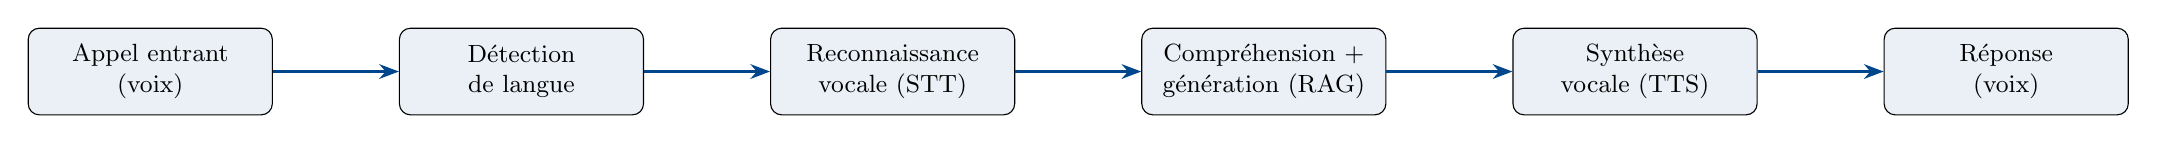
\begin{tikzpicture}[
    node distance=0.9cm and 1.6cm,
    box/.style={draw, rounded corners, fill=esprit!8, minimum width=3.1cm, minimum height=1.1cm, align=center, font=\small},
    arr/.style={-{Stealth[length=2.5mm]}, thick, esprit}
]
\node[box] (voix1) {Appel entrant\\(voix)};
\node[box, right=of voix1] (lang) {Détection\\de langue};
\node[box, right=of lang] (stt) {Reconnaissance\\vocale (STT)};
\node[box, right=of stt] (rag) {Compréhension +\\génération (RAG)};
\node[box, right=of rag] (tts) {Synthèse\\vocale (TTS)};
\node[box, right=of tts] (voix2) {Réponse\\(voix)};

\draw[arr] (voix1) -- (lang);
\draw[arr] (lang) -- (stt);
\draw[arr] (stt) -- (rag);
\draw[arr] (rag) -- (tts);
\draw[arr] (tts) -- (voix2);
\end{tikzpicture}
\end{center}

\begin{center}
\begin{tabular}{@{}p{4.2cm}p{9.5cm}@{}}
\toprule
\textbf{Module} & \textbf{Statut} \\
\midrule
Détection de langue (FR / arabe tunisien) & \textbf{Fait} -- \texttt{faster-whisper}, 100\% local \\
Reconnaissance vocale (STT) & \textbf{Fait} -- \texttt{faster-whisper} (medium), testé \\
Compréhension de la question (LLM) & \textbf{Fait} -- intégrée au module RAG \\
Génération de réponses (RAG) & \textbf{Fait} -- testé et amélioré (voir chap.~\ref{chap:rag}) \\
Synthèse vocale (TTS) & \textbf{Fait} -- Piper, voix française \\
API REST (backend) & \textbf{Fait} -- 5 endpoints fonctionnels \\
Dashboard (CRUD + stats/KPI) & \textbf{Non commencé} \\
Docker (conteneurisation + déploiement) & \textbf{Non commencé} \\
\bottomrule
\end{tabular}
\end{center}

\section{Récapitulatif des modèles utilisés}

\begin{center}
\begin{longtable}{@{}p{4cm}p{4cm}p{6cm}@{}}
\toprule
\textbf{Étape} & \textbf{Modèle / outil} & \textbf{Détails} \\
\midrule
\endhead
Détection de langue & \texttt{faster-whisper} (medium) & Même modèle que le STT (partagé
en mémoire), CPU, quantification int8 \\
Reconnaissance vocale (STT) & \texttt{faster-whisper} (medium) & 100\% local,
\texttt{device=cpu}, \texttt{compute\_type=int8} \\
Embeddings (recherche RAG) & \texttt{sentence-transformers} \newline
(\texttt{paraphrase-multilingual-mpnet-base-v2}) & Multilingue français + arabe, local \\
Base vectorielle (RAG) & ChromaDB & Stockage des embeddings, persisté dans
\texttt{vector\_store/} \\
Génération de réponse (RAG/LLM) & Ollama \newline (\texttt{qwen2.5:7b-instruct}) & 7
milliards de paramètres, 50\%/50\% CPU/GPU (VRAM limitée à 4~Go) \\
Synthèse vocale (TTS) & Piper \newline (\texttt{fr\_FR-siwis-medium}) & Français
uniquement, 100\% local \\
\bottomrule
\end{longtable}
\end{center}

Tous ces modèles sont \textbf{gratuits, open-source, et tournent entièrement en local}
(aucune clé API), conformément à la contrainte fondamentale du projet (voir
section~1.2).

\section{Structure du dépôt}
\begin{verbatim}
data/                    Collecte et preparation de la base de connaissances
  raw_data/              Documents bruts (PDF, pages HTML scrapees)
  processed/             Base de connaissances nettoyee (site_esprit_clean.json)
  scripts/               Scripts de scraping, extraction PDF, nettoyage

modules/
  rag/                   Generation de reponses (RAG)
  language_detection/    Detection francais / arabe
  speech_to_text/        Reconnaissance vocale
  text_to_speech/        Synthese vocale

backend/                 API REST reliant les modules
  routers/               rag.py, stt.py, tts.py
extraction_app/          Appli separee : ingestion controlee de nouvelles
                          fiches dans site_esprit.json (PDF/Excel/image/URL)
dashboard/               (a venir)
docker/                  (a venir)
tests/                   Scripts de test manuels
voice_models/            Modeles de voix Piper (gitignore, telechargeable)
vector_store/            Base vectorielle ChromaDB (gitignore, regeneree)
\end{verbatim}

\chapter{Infrastructure et environnement}

\section{Migration du disque C vers le disque D}
Le projet a été déplacé du disque C: vers le disque D: (\texttt{d:\textbackslash
stage\_ia\_recepsionist}) par manque d'espace sur C. Les caches de modèles ont été
redirigés vers D via des variables d'environnement Windows persistantes :
\begin{itemize}
    \item \texttt{OLLAMA\_MODELS} = \texttt{D:\textbackslash ai\_cache\textbackslash
    ollama\_models\textbackslash models}
    \item \texttt{HF\_HOME} = \texttt{D:\textbackslash ai\_cache\textbackslash
    huggingface} (cache Hugging Face : embeddings + Whisper)
\end{itemize}

\begin{noteinfo}
\textbf{Piège identifié} : un terminal déjà ouvert avant la création de la variable
d'environnement ne la voit pas (les variables \texttt{User} ne sont lues qu'au démarrage
d'un nouveau process). Toujours ouvrir un terminal neuf, ou refaire
\texttt{\$env:HF\_HOME = "D:\textbackslash ai\_cache\textbackslash huggingface"}
manuellement si un téléchargement inattendu se déclenche.
\end{noteinfo}

\section{Cause réelle de l'espace disque C qui se remplissait}
Contrairement à l'hypothèse initiale (les modèles IA), la vraie cause identifiée est
double :
\begin{enumerate}
    \item \textbf{Docker Desktop} : les disques virtuels WSL2 (\texttt{docker\_data.vhdx}
    $\approx$ 8,7~Go et \texttt{ext4.vhdx} $\approx$ 3,5~Go) vivent sur C par défaut et ne
    rétrécissent jamais automatiquement. Solution proposée (pas encore appliquée) :
    déplacer l'emplacement du disque Docker vers D.
    \item \textbf{Fichiers système Windows} : \texttt{pagefile.sys} ($\approx$ 19~Go) et
    \texttt{hiberfil.sys} ($\approx$ 6,3~Go), gonflés par la pression mémoire (16~Go de
    RAM, forte utilisation par Whisper + Ollama + Docker simultanément). Solution
    proposée : déplacer le fichier d'échange vers D via les paramètres de performance
    Windows (nécessite droits admin + redémarrage).
\end{enumerate}

\section{Matériel et limites de performance}
\begin{itemize}
    \item GPU : NVIDIA GeForce GTX 1650 Ti, \textbf{4~Go de VRAM seulement}.
    \item Ollama (modèle 7B) tourne en partage \textbf{50\% CPU / 50\% GPU} (le modèle ne
    tient pas entier dans la VRAM).
    \item Whisper (STT) tourne \textbf{entièrement en CPU}, décision volontaire pour ne
    pas entrer en conflit de VRAM avec Ollama (voir
    \texttt{modules/speech\_to\_text/config.py}).
    \item Conséquence : \texttt{/api/converse} (cycle complet voix→voix) prend environ
    \textbf{20 à 40 secondes} par question, une fois les modèles chargés en mémoire (le
    tout premier appel après un redémarrage du serveur est plus lent : chargement des
    modèles en RAM).
\end{itemize}

\chapter{Module reconnaissance vocale et détection de langue}

\section{Choix techniques}
Basé sur \texttt{faster-whisper}, modèle \texttt{medium}, 100\% local et gratuit. Les
modules \texttt{speech\_to\_text} et \texttt{language\_detection} partagent le même
modèle chargé en mémoire (\texttt{modules/speech\_to\_text/model.py}) pour éviter de le
charger deux fois.

\section{Amélioration : biais de vocabulaire}
Un paramètre \texttt{INITIAL\_PROMPT} a été ajouté
(\texttt{modules/speech\_to\_text/config.py}) pour biaiser le décodage de Whisper vers le
vocabulaire du domaine (noms propres ESPRIT, termes admissions/scolarité) et quelques
tournures tunisiennes courantes (باش، نجم، فما، برشة). Coût nul, réversible, aucune
garantie universelle -- aide sur des mots spécifiques, pas sur la grammaire ou l'accent
en général.

\begin{statutlimite}
\textbf{Limite connue et documentée par la recherche} : Whisper (même en version
\texttt{large}) est entraîné très majoritairement sur de l'arabe standard et quelques
dialectes bien dotés en données (égyptien...). Le tunisien (derja) reste
sous-représenté. Des modèles communautaires dédiés existent
(\texttt{sadeemar/whisper-finetuned-Tunisian}, \texttt{SalahZa/Tunisian\_Automatic\_
Speech\_Recognition}) mais sans garantie de qualité supérieure vérifiée, ou avec un
changement d'architecture non négligeable (WavLM/SpeechBrain). Un fine-tuning maison
demanderait de collecter et annoter nos propres enregistrements tunisiens -- hors
périmètre réaliste du stage.
\end{statutlimite}

\section{Protocole de test qualité}
Un script dédié (\texttt{tests/test\_language\_quality.py}) guide l'utilisateur à travers
8 sujets représentatifs de la base de connaissances (admission, frais, paiement,
calendrier, stage, documents, contact général, hors-sujet), enregistre chaque réponse en
arabe tunisien, l'enchaîne dans le pipeline complet, et sauvegarde un rapport JSON
(\texttt{Bureau\textbackslash test\_arabe\_resultats.json}) pour analyse structurée.

\chapter{Module RAG (génération de réponses)}
\label{chap:rag}

\section{Architecture}
\begin{itemize}
    \item \textbf{Base vectorielle} : ChromaDB, persistée dans \texttt{vector\_store/}
    (regénérée via \texttt{python -m modules.rag.ingest}).
    \item \textbf{Embeddings} : \texttt{sentence-transformers}, modèle
    \texttt{paraphrase-multilingual-mpnet-base-v2} (multilingue FR/AR).
    \item \textbf{LLM} : Ollama, modèle \texttt{qwen2.5:7b-instruct} (bon support
    multilingue parmi les modèles open-source).
    \item \textbf{Seuil de pertinence} : \texttt{SCORE\_THRESHOLD = 0.45} -- en dessous,
    redirection vers un message de fallback (service humain).
\end{itemize}

\section{Amélioration 1 : détection d'ambiguïté entre programmes}
\textbf{Problème constaté} : une question vague (\emph{``combien ça coûte pour étudier à
ESPRIT ?''}) piochait dans la première fiche la mieux notée, sans vérifier qu'elle
correspondait bien au bon programme parmi plusieurs (cours du jour, cours du soir,
EMBA...). Exemple observé : réponse de 20~000~DT (tarif EMBA) au lieu des 8~000~DT du
programme d'ingénieur généraliste.

\textbf{Solution implémentée} (\texttt{modules/rag/programmes.py} +
\texttt{modules/rag/pipeline.py}) :
\begin{enumerate}
    \item Chaque fiche est associée à un \emph{programme} (cours du jour tunisiens /
    internationaux, cours du soir, EMBA, alternance...) déduit de son URL source.
    \item Si, parmi les meilleures fiches retrouvées (à une marge de score près), au
    moins deux programmes différents sont représentés \textbf{et} que la question ne
    précise pas lequel, le système répond directement par une demande de clarification
    -- \textbf{sans appeler le LLM} (quasi instantané, $\sim$0,3s au lieu de 15 à 40s).
    \item Garde-fou anti-faux-positif : la détection ne se déclenche que si le
    \emph{meilleur} résultat est déjà spécifique à un programme (sinon, une question sur
    un service général -- stage, carrière... -- ne serait pas concernée).
    \item Garde-fou supplémentaire : si la question mentionne déjà explicitement un
    programme par mot-clé (ex. ``cours du soir''), pas de clarification demandée.
\end{enumerate}

\textbf{Résultat validé} : questions précises (``frais des cours du soir'') répondent
normalement ; questions vraiment vagues (``comment puis-je payer ?'') déclenchent la
clarification ; questions sur des services généraux (``service de stage'') ne
déclenchent plus de faux positif.

\section{Amélioration 2 : qualité des données -- fiches ``gouvernance''}
\textbf{Problème constaté} : une question sur le département des stages ne mentionnait
jamais le contact réel (Majdi Gharbi) alors que l'information existait dans la base.

\textbf{Cause racine} : \texttt{modules/rag/ingest.py} embed le texte
\texttt{"\{titre\} : \{contenu\}"}. Pour les 28 fiches de la page gouvernance, le titre
était le \textbf{nom de la personne} (ex. ``Majdi GHARBI''), qui dilue l'embedding au lieu
de l'aider -- un nom propre n'apporte aucun signal utile à la recherche sémantique.

\textbf{Correction appliquée} (\texttt{data/processed/site\_esprit\_clean.json},
28 fiches) :
\begin{itemize}
    \item \textbf{Titre} : nom de la personne $\to$ sujet/département (ex.
    ``Département des stages'').
    \item \textbf{Contenu} : reformulé en phrase naturelle (ex. \emph{``Majdi GHARBI est
    la personne à contacter pour toute question sur département des stages. Email :
    majdi.gharbi@esprit.tn.''}).
    \item Base réindexée.
\end{itemize}

\textbf{Résultat mesuré} : score de similarité passé de absent du top 10 à 0{,}601 (2\textsuperscript{e}
position) sur la question ``qui contacter pour le département des stages ?''. La réponse
finale mentionne désormais correctement le contact.

\begin{noteinfo}
\textbf{Limite honnête} : la correction fonctionne pour les formulations proches du
vocabulaire de la fiche. Des formulations plus détournées (``je cherche un stage, qui
dois-je contacter ?'') ne remontent toujours pas cette fiche -- limite inhérente à la
recherche sémantique sur des textes courts.
\end{noteinfo}

\section{Amélioration 3 : extraction et regroupement du dossier Admission}
\textbf{Objectif} : les documents \texttt{.docx} de \texttt{data/raw\_data/Admission/}
(FAQ par programme, conseillers admission) n'étaient pas encore dans la base de
connaissances. Plutôt que d'indexer une fiche par question isolée, le contenu est
\textbf{regroupé par section} (titres en gras du document, ex. ``Admission et
Inscription'', ``Modalités Financières'') : ni trop court (une seule question, mal
retrouvée en recherche sémantique -- voir amélioration 2), ni trop long (dilution de
l'embedding sur plusieurs sujets différents).

\textbf{Script} : \texttt{data/scripts/extract\_admission\_docx.py} -- analyseur souple
gérant plusieurs variantes de mise en forme (question/réponse en paragraphes séparés ou
combinés, sections purement descriptives), avec nettoyage des notes d'auteur parasites
(ex. ``(mettre 3 boutons cliquables...)''). Chaque fiche est rattachée au bon programme
(réutilisation des URLs canoniques déjà utilisées par le système de détection
d'ambiguïté, section~\ref{chap:rag}).

\textbf{Résultat} : 27 fiches ajoutées (785 fiches au total avant l'audit ci-dessous),
comparées à \texttt{site\_esprit\_clean.json} existant (aucun doublon exact). Test sur
une question vague (``comment ça marche l'inscription aux cours du soir ?'') : réponse
complète en 5 étapes -- bonne, mais pas systématiquement grâce aux nouvelles fiches
précises (beaucoup de contenu existant fait concurrence en recherche).

\section{Audit de la base de connaissances : fiches peu détaillées ou hors-sujet}
Un audit systématique (fiches de moins de 60 caractères, 86 sur 785) a révélé plusieurs
catégories de problèmes :
\begin{enumerate}
    \item \textbf{Conflit de calendriers} ($\sim$60 fiches) : trois fichiers calendrier
    différents (1,2,3\&4A / 5A / 5DS9\&5Infini3) avec des dates différentes pour des
    événements similaires (ex. vacances d'hiver) -- risque de réponse mélangeant les
    années/promotions. \textbf{Pas encore corrigé.}
    \item \textbf{Bruit PDF hors-sujet} : le document \texttt{RDI\_CATALOG\_2023-2024.pdf}
    (rapport annuel de recherche académique -- équipes de recherche, publications
    scientifiques, conférences) s'est révélé \textbf{entièrement hors périmètre} pour un
    assistant de réception admissions/scolarité. \textbf{Corrigé} : 49 fiches supprimées
    (785 $\to$ 736 fiches), base réindexée, aucune régression constatée (une des
    nouvelles fiches ``Modalités Financières'' est même remontée en 1\textsuperscript{re}
    position sur un test déjà validé, probablement grâce à moins de contenu parasite en
    concurrence).
    \item \textbf{Fiches contact avec nom en titre} (ex. ``Ramla Ben Ouirane'', ``Pr.
    Faouzi Kamoun'') : même défaut que la correction ``Département des stages''
    ci-dessus. \textbf{Pas encore corrigé.}
    \item \textbf{Lignes de grille tarifaire isolées} (ex. ``550DT'' / ``Demi-pension
    (F1)...'') : extraites une par une sans le contexte du tableau d'origine. Lié au
    sous-dossier \texttt{Admission/Grilles tarifaires/} (PDF, Excel, zip), \textbf{pas
    encore traité}.
\end{enumerate}

\section{Nettoyage : préfixe d'interface web et doublons de contenu}
Deux problèmes supplémentaires, découverts en creusant le mécanisme même de la
recherche sémantique (comment le RAG choisit une fiche pour une question donnée) :

\textbf{1. Préfixe d'interface parasite} : 85 fiches sur 736 avaient un titre commençant
par \emph{``Ouvrir la visibilité du contenu : ''} -- le libellé du bouton ``déplier'' d'un
accordéon FAQ, scrapé par erreur avec la vraie question. Comme
\texttt{modules/rag/ingest.py} donne du poids au titre dans l'embedding, ce préfixe
identique sur 85 fiches diluait leur pertinence. \textbf{Corrigé} : préfixe retiré
(regex simple, aucun risque -- ne touche jamais le contenu factuel).

\textbf{2. Doublons de contenu préexistants, révélés par le nettoyage} : une fois les
titres nettoyés, ces fiches ont mieux remonté en recherche -- révélant que
\textbf{4 groupes de fiches quasi-identiques} existaient déjà entre plusieurs pages de
programmes (ex. ``Les diplômes délivrés par ESPRIT sont-ils reconnus ?'' dupliqué mot
pour mot entre les pages ``cours-du-jour-tunisiens'' et ``cours-du-jour-internationaux'').
Conséquence concrète : le système de détection d'ambiguïté (section~\ref{chap:rag})
demandait à tort de préciser le programme, alors que la réponse est identique quel que
soit le programme choisi. \textbf{Corrigé} : les 4 groupes fusionnés en une seule fiche
chacun, retaguée avec une source générique non rattachée à un programme spécifique
(736 $\to$ 730 fiches). Testé et validé : la question ``le diplôme ESPRIT est-il
reconnu ?'' répond désormais directement, sans fausse demande de clarification.

\begin{noteinfo}
Cet épisode illustre bien la nature itérative du nettoyage de données pour un RAG :
corriger un problème (préfixe parasite) peut révéler un autre problème resté invisible
jusque-là (doublons), simplement parce que les fiches concernées remontent différemment
en recherche une fois nettoyées.
\end{noteinfo}

\section{Clôture de l'audit : les 4 chantiers restants traités}

\textbf{1. Fiches contact restantes} : 2 dernières fiches avec un nom de personne en
titre (``Ramla Ben Ouirane'', ``Pr. Faouzi Kamoun'') corrigées selon le même schéma que
``Département des stages''. La fiche du centre de carrière a ensuite été reformulée une
seconde fois (titre sous forme de question ``Qui contacter au centre de carrière ?'')
après un test montrant qu'elle perdait face à des FAQ génériques ``qui contacter''
d'autres programmes.

\textbf{2. Conflit des calendriers} : les 67 fiches issues des 3 fichiers calendrier
(1,2,3\&4A / 5A / 5DS9\&Infini3) sont désormais préfixées avec leur promotion
(ex. \emph{``Pour 5ème année (5A) -- le mardi 2025-12-30 : Vacances d'hiver.''}) : même si
plusieurs dates concurrentes remontent en recherche, la réponse ne peut plus mélanger les
promotions.

\textbf{3. Grilles tarifaires} (\texttt{Admission/Grilles tarifaires/}) : 7 PDF + 1 Excel
extraits avec \texttt{pdfplumber} en mode \emph{tableau} (pas texte brut, pour ne pas
mélanger les colonnes). Le fichier zip du dossier s'est révélé être une copie exacte de 4
PDF déjà présents (tailles de fichier identiques) -- ignoré. 10 fiches ajoutées : foyer et
restauration (tunisiens/internationaux), historique des frais 2018-2025 (cours du jour et
cours du soir), classe préparatoire (PREPA, nouveau programme ajouté au système de
détection d'ambiguïté), et ESPRIT School of Business (Bachelor/Master). Chaque montant a
été vérifié manuellement contre le tableau source avant d'être transcrit en phrase
complète -- aucune réécriture automatique de chiffres.

\textbf{4. Champs \texttt{source} et \texttt{type}} : vérifié dans le code que ni l'un ni
l'autre n'est jamais envoyé au LLM ni à l'embedding (\texttt{ingest.py} et
\texttt{generator.py} n'utilisent que \texttt{titre} + \texttt{contenu}). \texttt{type}
était réellement mort code (jamais relu) -- supprimé de toutes les fiches et des 6 scripts
d'extraction. \texttt{source} est en revanche activement utilisé par la détection
d'ambiguïté et les citations -- conservé. Le vrai risque de confusion identifié était
ailleurs : \textbf{203 fiches} avaient un titre brut de type
\emph{``nom-fichier.pdf - page N''} (ex. \texttt{Reglement-scolarite-24-25-cs.pdf - page
8}), qui pollue l'embedding (titre pesé dans la recherche). Un test empirique a confirmé
qu'un titre nettoyé (ex. \emph{``Règlement de la scolarité - Cours du soir
2024-2025''}) score mieux (0,667) qu'un titre brut (0,659) et qu'une absence de titre
(0,654) -- les 203 titres ont été remappés vers des noms lisibles pour les 18 documents
concernés.

\textbf{5. Robustesse de la détection d'ambiguïté} : un cas limite a révélé que la règle
``ne se déclenche que si le meilleur résultat a un label'' était fragile -- un écart de
score de 0{,}001 entre deux fiches (bruit d'embedding) suffisait à faire basculer une
question générale (``comment fonctionne le service de stage ?'') en fausse alerte.
\textbf{Corrigé} : la règle regarde maintenant un consensus sur les 3 meilleurs résultats
(majorité avec un label de programme) plutôt que le seul premier résultat -- plus robuste
au bruit, sans perdre la détection des vrais cas ambigus.

Base de connaissances finale : \textbf{740 fiches} (730 avant ce chantier, +10 fiches de
grilles tarifaires). Régression complète validée sur 5 scénarios de référence (précis /
vague / général / contact / calendrier) avant clôture de ce chantier.

\section{Correction : cul-de-sac de la clarification en mode vocal}
\textbf{Problème découvert en testant} \texttt{/api/converse} \textbf{avec une vraie
voix} : sur une question vague (``comment puis-je payer ?''), l'appelant recevait la
demande de clarification (``précisez le programme'') \emph{en audio}, sans aucun moyen
d'y répondre -- \texttt{/api/converse} est un aller-retour unique (audio $\to$ audio),
sans mémoire de conversation entre deux appels. Demander une précision qu'on ne peut pas
recevoir est un cul-de-sac inacceptable en usage téléphonique réel.

\textbf{Correction} : \texttt{answer\_question()} accepte désormais un paramètre
\texttt{allow\_clarification} (\texttt{modules/rag/pipeline.py}). Quand il vaut
\texttt{False}, le LLM génère toujours une réponse directe même en cas d'ambiguïté
détectée -- une note est ajoutée au prompt (\texttt{modules/rag/generator.py}) lui
demandant de couvrir les principaux programmes concernés plutôt que de refuser de
répondre.

Après test, décision prise d'appliquer ce comportement \textbf{uniformément aux 3
endpoints} (\texttt{/api/ask}, \texttt{/api/voice-ask}, \texttt{/api/converse}) : plus
aucune demande de clarification nulle part, pour une expérience cohérente quel que soit
le canal.

Testé : la même question ambiguë donne désormais une réponse directe et utile sur les 3
endpoints (ex. détail des tranches de paiement pour plusieurs programmes, avec une
invitation à vérifier les spécificités de son propre programme), au lieu d'une question
sans issue.

\section{Nettoyage : catégorie ``Vie étudiante''}
\textbf{Problème signalé} : la catégorie ``Vie étudiante'' (144 fiches) contenait
beaucoup de détail et plusieurs fiches jugées inutiles. Analyse : 103 des 144 fiches
étaient en réalité des \textbf{règlements de scolarité mal catégorisés} (laissés
intacts, car potentiellement utiles pour de vraies questions réglementaires) ; les
41 fiches restantes (clubs, alumni, étudiants internationaux, cellule d'écoute)
constituaient la vraie ``vie étudiante'', ciblée par ce nettoyage.

\textbf{Supprimé (9 fiches, aucune valeur informative)} :
\begin{itemize}
    \item 6 fiches ``Visite virtuelle'' : légendes marketing génériques sans même le nom
    de la salle décrite (ex. ``un espace calme et inspirant'').
    \item 2 fiches ``Règlement intérieur'' : renvoyaient simplement à ``télécharger le
    règlement ailleurs'', sans contenu réel.
    \item 1 fiche fusionnée avec une autre (cellule d'écoute, partie 2/2 courte).
\end{itemize}

\textbf{Raccourci (32 fiches : 20 clubs, 3 alumni, 6 étudiants internationaux, 3 cellule
d'écoute)} : style promotionnel/verbeux retiré, tous les faits conservés (emails,
téléphones, adresse, dates de fondation). Médiane de longueur : 821 $\to$ 167 caractères.

\begin{noteinfo}
\textbf{Erreur de données trouvée et corrigée au passage} : la fiche ``Cellule d'écoute''
contenait une phrase sur la communauté Alumni, copiée par erreur depuis une autre page
lors du scraping initial -- retirée car factuellement fausse dans ce contexte.
\end{noteinfo}

Testé : question sur un club (robotique) $\to$ bon club identifié avec email (score
0,722) ; question de détresse psychologique (formulation naturelle) $\to$ cellule
d'écoute remontée en premier avec coordonnées complètes.

\section{Consolidation par sujet : facilités de paiement}
\textbf{Demande} : quand la question porte sur un sujet transversal (ex. ``puis-je payer
par facilité ?''), la réponse doit couvrir toutes les méthodes existantes, pas une seule
au hasard parmi des doublons.

\textbf{Constat} : le paragraphe ``Financement'' (prêt Fondation ESPRIT, banques
partenaires Amen/Zitouna/UBCI, jusqu'à 36 mensualités) était dupliqué quasi à l'identique
sur \textbf{6 fiches différentes} (plusieurs pages de grilles tarifaires, années
2024-2025 et 2025-2026). Avec seulement 5 fiches remontées par requête
(\texttt{TOP\_K}), 4 des 5 places pouvaient être occupées par la même information
répétée, au détriment d'informations réellement différentes (ex. le financement
spécifique à l'EMBA : 2 à 5 tranches, partenariat Banque Zitouna).

\textbf{Corrigé} : les 6 doublons remplacés par une fiche unique ``Facilités de paiement
et financement (tous programmes)'', couvrant le cas général (cours du jour/soir) et le
cas EMBA côte à côte.

\section{Consolidation par sujet : réductions sur les frais de scolarité}
\textbf{Constat} : l'information sur les réductions (mérite académique, fratrie, cours du
soir) était éparpillée sur une douzaine de fiches (FAQ générale, pages Admissions
spécifiques par programme, fiches Paiements 2024-2025), avec des taux légèrement
différents selon la fiche (25\%/10\% ici, 30\%/15\% là) sans qu'il soit évident qu'il
s'agissait en réalité de la même politique exprimée sous forme de fourchettes
(``excellence haute'' 25--30\%, ``excellence standard'' 10--15\%) plutôt que de valeurs
contradictoires. Aucune fiche ne couvrait le cas des étudiants internationaux (plafonds
30\%/40\%), la règle de non-cumul, ni la procédure de demande (dossier conjoint signé par
les tuteurs + copies des cartes d'identité).

\textbf{Corrigé} : ajout d'une fiche unique consolidée (\texttt{paiements\_reductions\_}
\texttt{scolarite\_detail\_complet}) couvrant les quatre volets (mérite, fratrie, cours du
soir, conditions générales/démarche) à partir d'informations internes confirmées. Les
fiches existantes (issues du site, déjà validées) n'ont pas été supprimées -- elles
restent cohérentes avec la nouvelle fiche (leurs taux sont des cas particuliers dans les
fourchettes données), seulement incomplètes prises isolément.

\begin{noteinfo}
Test de bout en bout après ré-indexation (\texttt{python -m modules.rag.ingest}) : la
nouvelle fiche remonte en premier ($\text{score}=0.876$) sur la question ``Quelles sont
les réductions possibles sur les frais de scolarité ?''. La réponse générée reste
volontairement concise (persona vocal, \texttt{SYSTEM\_PROMPT} impose des ``réponses
courtes et naturelles à l'oral'') et ne récite donc pas exhaustivement tous les
pourcentages -- comportement voulu pour un appel téléphonique, mais qui mérite d'être
validé avec l'utilisateur si le besoin réel est une réponse plus détaillée pour ce type de
question transversale.
\end{noteinfo}

\section{Nouvelle fiche : attestations et relevé de notes}

Ajout d'une fiche FAQ (\texttt{faq\_attestation\_presence\_reussite\_releve\_notes}) sur
la procédure pour obtenir une attestation de réussite, une attestation de présence ou un
relevé de notes -- information communiquée directement par l'utilisateur (contact par
email au service des élèves correspondant à la classe, une adresse par année de
1\textsuperscript{re} à 5\textsuperscript{e}, puis passage au bureau du service des
élèves trois jours après l'envoi). Vérifié : aucune fiche existante ne couvrait déjà ce
sujet, pas de risque de doublon.

\section{Écart de vocabulaire : ``conseil de classe'' vs libellés calendrier}

\textbf{Constat} : la question ``Quelle est la date des conseils de classe ?'' ne
remontait \textbf{aucune} des fiches calendrier pertinentes (meilleur score 0{,}69, sur
une fiche totalement hors-sujet), alors que la question ``Quelle est la date du conseil
de la session principale ?'' fonctionnait (score 0{,}765). Cause : les 4 fiches
calendrier concernées utilisent exclusivement les libellés bruts du PDF source
(``Conseils Session Principale'', ``Conseils de la session principale'') et ne
contiennent jamais le mot ``classe'' -- le terme générique que les appelants utilisent
naturellement n'existe nulle part dans le texte embeddé de ces fiches.

En vérifiant les PDF sources (\texttt{pdfplumber}, avant toute correction) : le libellé
``Conseils de la session principale'' apparaît bien deux fois à l'identique dans
\texttt{Calendrier\_5DS9 \& 5INFINI3.pdf} (16 et 30 janvier) -- confirmé fidèle au PDF,
pas une erreur d'extraction, donc non modifié. En revanche, la coquille ``Session de
rattraoage'' (pour ``rattrapage'') est également confirmée présente telle quelle dans le
PDF source (\texttt{Calendrier\_5A\_ 2526\_S1.pdf}) -- corrigée dans la base car elle
nuit à la recherche sans changer le sens.

\textbf{Corrigé} : les 4 fiches calendrier mentionnant un conseil (2 pour 5ème année/5A,
2 pour 5DS9/5Infini3) enrichies pour inclure explicitement ``conseil de classe'' en
titre et contenu, en plus du libellé original conservé.

\begin{statutfait}
Test après ré-indexation : la question ``conseils de classe'' fait maintenant remonter
les deux fiches 5A (scores 0{,}679 et 0{,}635) et la réponse générée donne correctement
les deux dates (3 décembre : session principale, 24 décembre : rattrapage). Point de
vigilance : les scores restent inférieurs à certains résultats hors-sujet (0{,}69/0{,}68)
-- la correction fonctionne mais reste proche du seuil, une base plus large de synonymes
(ex. mentionner aussi ``conseil de classe'' dans les fiches 1\textsuperscript{re} à
4\textsuperscript{e} année si un tel évènement existe dans leur calendrier) resterait à
vérifier si le problème réapparaît sur d'autres formulations.
\end{statutfait}

\section{Refonte complète des calendriers : extraction groupée par type d'événement}

\textbf{Demande} : l'ancienne extraction (\texttt{data/scripts/extraction\_calendrier.py})
produisait une fiche minuscule par événement individuel (une par jour), jugée
insatisfaisante. Un nouveau fichier a par ailleurs été ajouté
(\texttt{Calendrier du deuxième semestre\_2526.pdf}), à intégrer également.

\textbf{Nouveau script} : \texttt{data/scripts/reextract\_calendrier\_groupe.py}.
Reprend la reconstruction de date fiable (extraction de tableaux \texttt{pdfplumber},
déjà éprouvée), mais regroupe les événements par \textbf{type}
(rentrée/débuts de semestre, APP0, examens session principale, examens session de
rattrapage, conseils de classe, proclamation des résultats, fin des cours, vacances,
soutenances, autres) plutôt qu'un par jour -- une seule fiche cohérente par (groupe
d'année × type) listant toutes les dates correspondantes.

\begin{statutlimite}
\textbf{Bug d'extraction découvert et corrigé} : en inspectant la structure brute des
tableaux \texttt{pdfplumber} (pas seulement le texte à plat), certains événements dont
le libellé est trop long pour une seule case (ex. ``Examens de la Session de
Rattrapage'') débordent visuellement sur la case du jour \textbf{suivant} dans le PDF
source -- \texttt{pdfplumber} attribue alors à tort le second morceau de texte
(``Rattrapage'' seul) à ce jour suivant, créant deux évènements fantômes tronqués au
lieu d'un seul événement complet correctement daté. Corrigé par une fusion des
fragments de continuation reconnus (\texttt{CONTINUATION\_FRAGMENTS}) avec l'événement
de la veille, quand les deux jours sont consécutifs. Egalement filtrés : les numéros de
semaine (``S1'' à ``S16'') affichés dans la grille, qui ne sont pas de vrais événements.
\end{statutlimite}

\begin{statutfait}
Les 45 anciennes fiches ``Calendrier*'' supprimées de \texttt{site\_esprit\_clean.json}
et \texttt{site\_esprit.json}, remplacées par 34 fiches regroupées (ajoutées en fin de
fichier). Après ré-indexation, trois questions testées avec de bons scores : date de
l'APP0 (0{,}783), début des études 5ème année (0{,}751), conseils de classe (0{,}771 --
contre 0{,}679 avec la version précédente, et 0{,}69 sur une fiche hors-sujet avant tout
correctif). La réponse sur les conseils de classe mentionne aussi correctement l'absence
de date pour les années 1\textsuperscript{re} à 4\textsuperscript{e} (vérifié : ce
calendrier ne contient effectivement aucun événement ``conseil'').
\end{statutfait}

\section{Confirmation utilisateur : le calendrier semestre 2 est commun à tous les groupes}

Point laissé ouvert plus haut : confirmé par l'utilisateur que
\texttt{Calendrier du deuxième semestre\_2526.pdf} s'applique de la même façon aux 5
groupes d'année (1\textsuperscript{re} à 5\textsuperscript{e}), malgré l'absence de
qualificatif dans son titre. Les événements de ce fichier sont donc désormais fusionnés
dans les fiches de \textbf{chacun} des 3 groupes existants (au lieu d'une catégorie à
part), avec la source combinée des deux fichiers d'origine par fiche concernée.

\begin{statutlimite}
\textbf{Bug de génération découvert en aval} : même après cette fusion, la question
``Quand commence la session de contrôle pour les 1ère année ?'' produisait toujours une
réponse vague et non sourcée (``généralement en février ou mars... vérifiez le site
web''), alors que la fiche pertinente était bel et bien récupérée (2\textsuperscript{e}
sur 5 sources, score 0{,}692) -- le LLM ne faisait simplement pas le lien entre
``session de contrôle'' (terme de l'utilisateur) et ``session de rattrapage'' (terme
utilisé dans la fiche), et ignorait cette source dans sa réponse malgré sa présence dans
le contexte fourni. Corrigé par le même type de synonyme explicite que pour ``conseil de
classe'' : les fiches de type rattrapage portent désormais aussi la mention ``(session
de contrôle)''.
\end{statutlimite}

\begin{statutfait}
Après ce correctif et une nouvelle ré-indexation : la fiche concernée remonte en
\textbf{premier} résultat (score 0{,}706, contre 2\textsuperscript{e} position à 0{,}692
avant), et la réponse générée cite désormais une vraie date de la base (``la session de
contrôle commencera le mercredi 24 juin 2026'') au lieu d'une réponse générique inventée.
\end{statutfait}

\section{Règlements de scolarité : ré-extraction par article}
\textbf{Constat le plus important de cette session} : les 103 fiches de règlement
(cours du jour, cours du soir, alternance, Private School en anglais) étaient en réalité
des \textbf{pages brutes de PDF} (une fiche = une page, 100 à 2000 caractères), et non
des fiches organisées par sujet -- une page pouvant couper un article en plein milieu
ou mélanger la fin d'un article et le début du suivant. Cause : ces 4 documents avaient
été traités par le scraper web générique (extraction page par page), qui ignore la
structure ``Article N : Titre'' pourtant bien présente dans les PDF sources.

\textbf{Correction} : nouveau script \texttt{data/scripts/reextract\_reglements.py},
qui réextrait les 4 documents en respectant leur structure par article :
\begin{itemize}
    \item Découpage sur le motif \texttt{Article N :}, suppression du sommaire (table
    des matières) et des lignes de sommaire à pointillés (ASCII \texttt{.} ou ellipses
    unicode \texttt{…}) qui polluaient certains articles.
    \item Les articles trop longs (ex. ``Régime des examens'', ``Charte de l'étudiant'',
    8~000 à 13~700 caractères -- ils regroupent des sous-clauses non numérotées) sont
    sous-découpés en parties de 2000 caractères maximum, comme pour les autres documents
    du projet.
    \item Dédoublonnage des titres d'article répétés par erreur dans le PDF source.
\end{itemize}

\textbf{Doublon supplémentaire découvert et supprimé} : 23 fiches ``cours du jour''
existaient déjà, issues d'une extraction antérieure non documentée (source = nom de
fichier local, sans URL) -- contenu identique à la nouvelle extraction, supprimées au
profit de la version cohérente avec le reste de la base (source en URL \texttt{https://}).

\textbf{Résultat} : 103 fiches fragmentées $\to$ \textbf{88 fiches cohérentes par
article et par parcours}. Base de connaissances finale : \textbf{685 fiches}. Testé :
question sur les conditions d'obtention du diplôme (cours du jour) $\to$ score de
pertinence 0,782 (contre absence de structure claire avant), réponse complète et exacte
citant l'article source.

\section{Test qualité sur 35 questions et corrections}
\label{sec:test-qualite-35}
Un test systématique sur 35 questions couvrant 6 catégories (paiements, calendrier,
règlements, admissions, vie étudiante, questions pièges) a été mené via
\texttt{answer\_question()} directement (script \texttt{\_test\_batch\_questions.py},
temporaire). Deux problèmes réels ont été détectés et corrigés :

\textbf{1. Mauvaise identité du directeur.} À la question ``quel est le nom du directeur
actuel d'ESPRIT ?'', le modèle répondait \emph{Lamjed Bettaieb (Directeur Général
Adjoint)} au lieu du vrai Président-Directeur Général, \emph{Tahar Ben Lakhdar}. Cause :
9 fiches de gouvernance différentes (``Directeur administratif et financier'',
``Directeur des études'', ``Directeur Général Adjoint''...) contiennent toutes le mot
générique ``Directeur'' et scorent de façon quasi identique (0,475 à 0,561) -- le LLM,
recevant les 5 meilleures sans distinction claire de hiérarchie, ne priorisait pas le
Président-Directeur Général. \textbf{Corrigé} : ajout d'une fiche dédiée ``Qui est le
directeur de l'école ESPRIT ?'' répondant sans ambiguïté -- score de similarité 0,656
(nettement au-dessus des 9 fiches concurrentes), résout le cas.

\textbf{2. Réponse totalement corrompue (bug sévère).} À la question ``combien de fois
je peux redoubler ?'', le modèle générait un texte \textbf{en chinois}, sans rapport
avec la question (une conversation inventée sur la météo). Cause : le score de la
meilleure fiche récupérée n'était que 0,451 (à peine au-dessus du seuil de fallback
0,45), noyé parmi des fragments de prix totalement hors-sujet (``20~000 DT TTC'',
``3~200DT''...) -- le vrai fait (\emph{``le redoublement n'est toléré qu'une seule fois
par cycle de formation''}) existait bien dans la base mais enfoui dans un article de
règlement de 1856 caractères, mal capté par la recherche sémantique. \textbf{Corrigé} :
ajout d'une fiche dédiée consolidant les 3 parcours, avec une phrase de désambiguïsation
explicite (``un seul redoublement au total est autorisé, jamais deux'') après qu'une
première version ait fait dire au LLM ``deux redoublements'' par mauvaise lecture d'une
formulation par-parcours. Score final : 0,536 (validé empiriquement avant mise en
production, comme pour les autres corrections de ce rapport).

\begin{noteinfo}
\textbf{Leçon retenue} : un score de similarité proche du seuil de fallback (0,45) est
un signal fiable de risque de génération de mauvaise qualité, y compris des dérives
complètes (langue incorrecte, hors-sujet) -- pas seulement des réponses imprécises. À
surveiller pour d'éventuels ajustements futurs du seuil ou de garde-fous sur la
génération.
\end{noteinfo}

\section{Contradictions entre sources sur les frais 2024-2025}
Un script de nettoyage externe (non écrit dans cette session) proposait de supprimer les
fiches issues d'un email de paiement, jugées ``fausses'' par rapport à la grille
tarifaire du site. Vérification avant exécution -- deux cas distincts :

\textbf{Cas 1 (résolu par suppression)} : 4 fiches (\texttt{admissions\_cours\_du\_jour\_
tunisiens\_003} à \texttt{006}, valeurs de 2ème tranche par année) ne correspondaient pas
exactement à la fiche historique sourcée depuis le PDF officiel de grille tarifaire (3
des 4 valeurs différaient de 50 à 100 DT). Contrairement à ce qu'affirmait le script, ce
n'étaient pas des doublons identiques -- mais le PDF officiel étant plus fiable qu'une
page web potentiellement obsolète, les 4 fiches ont été supprimées.

\textbf{Cas 2 (résolu par clarification, pas suppression)} : le taux de réduction pour
mérite académique différait entre l'email (30\%/15\%) et le site (25\%/10\%). Lecture
attentive du contenu du site : celui-ci précise explicitement que le taux 25\%/10\% est
\emph{nouveau et applicable aux frais de 2025-2026}, décidé pendant l'année 2024-2025.
Le taux de l'email est donc probablement correct pour 2024-2025, pas une erreur. Les deux
valeurs ont été \textbf{conservées}, avec les titres clarifiés par année plutôt que l'une
supprimée au profit de l'autre.

\textbf{Cas 3 (non tranché, signalé pour vérification humaine)} : le montant total des
frais 2024-2025 diffère aussi (8200 DT selon l'email vs 8400 TND selon le site et une FAQ
docx). Contrairement au cas 2, \textbf{aucune des fiches ne mentionne de réserve
d'année} -- les deux affirment ce montant pour la même année 2024/2025 sans nuance.
Faute de moyen de vérifier laquelle est correcte, \textbf{aucune fiche n'a été supprimée
ni fusionnée} : les deux valeurs restent dans \texttt{site\_esprit\_clean.json}, et le
conflit est documenté séparément dans \texttt{data/processed/conflits\_a\_verifier.json}
pour vérification manuelle auprès du service financier.

\begin{noteinfo}
\textbf{Principe appliqué} : ne jamais trancher automatiquement une contradiction de
données factuelles (montants, taux) sans preuve claire de laquelle est correcte --
soit clarifier par un facteur objectif retrouvé dans le contenu (ici, l'année
d'application), soit signaler explicitement pour vérification humaine plutôt que de
deviner.
\end{noteinfo}

\section{Test qualité sur 100 questions et confirmation des montants par email officiel}
Un second test systématique, sur 100 questions couvrant 10 catégories, a révélé que le
bug de dérive complète du LLM (section~\ref{sec:test-qualite-35}) n'était pas propre à
la question du redoublement : il est réapparu sur une question sans rapport (classe
préparatoire), confirmant qu'il s'agit d'un risque systémique lié à un score de
pertinence faible, pas d'un cas isolé. Deux autres réponses se sont révélées fausses ou
contradictoires (campus de Monastir, existence d'ESPRIT School of Business),à recouper
avec les catégories internes de programmes.

L'utilisateur a ensuite fourni les deux emails officiels de réinscription (2024-2025 et
2025-2026) envoyés par la Direction, résolvant définitivement le conflit du montant
total signalé plus haut : \textbf{8200 DT pour 2024-2025 est confirmé correct} (les
fiches affirmant 8400 TND, aujourd'hui corrigées, étaient fausses) ; \textbf{8350 TND
pour 2025-2026} est ajouté comme nouvelle donnée confirmée (4050 TND avant le
31/08/2025, 4300 TND avant le 15/01/2026), avec 7 moyens de paiement détaillés (en
ligne, Amen Bank, BIAT, chèque, sur place, prélèvement 10 mensualités, traite avalisée).

\textbf{Difficulté technique rencontrée et résolue} : les nouvelles fiches 2025-2026,
formulées de façon neutre, scoraient moins bien (0,68) que l'ancienne fiche 2024-2025
(0,85) pour une question portant explicitement sur 2025/2026 -- confirmation que les
embeddings distinguent mal les années pures, un chiffre à 4 chiffres se ressemblant
sémantiquement d'une année à l'autre. Corrigé en répétant l'année plusieurs fois dans le
contenu et en contrastant explicitement avec l'année précédente (``concerne
spécifiquement 2025/2026, différent de 2024/2025'') : score porté à 0,88, redevenant la
source la plus pertinente. Le \texttt{conflits\_a\_verifier.json} a été mis à jour pour
marquer ce conflit comme résolu.

\chapter{Module synthèse vocale (TTS)}

\section{Choix techniques}
Basé sur \textbf{Piper} (moteur de synthèse neuronale, 100\% local, gratuit, aucune clé
API). Voix française \texttt{fr\_FR-siwis-medium} installée dans \texttt{voice\_models/}
(gitignored, retéléchargeable).

\section{Réglage de la vitesse}
La voix par défaut parlait trop vite pour un usage téléphonique. Un paramètre
\texttt{SPEECH\_LENGTH\_SCALE = 1.25} (25\% plus lent) a été ajouté dans
\texttt{modules/text\_to\_speech/config.py}, appliqué via \texttt{SynthesisConfig} de
Piper.

\begin{statutlimite}
\textbf{Limite connue} : aucune voix arabe tunisienne (dialecte) disponible chez Piper --
seulement de l'arabe standard moderne. Le module reste donc pertinent uniquement pour le
français pour l'instant.
\end{statutlimite}

\chapter{Backend / API REST}

\section{Endpoints disponibles}
\begin{center}
\begin{longtable}{@{}p{3.2cm}p{10.5cm}@{}}
\toprule
\textbf{Endpoint} & \textbf{Description} \\
\midrule
\endhead
\texttt{GET /api/health} & Vérifie que l'API répond. \\
\texttt{POST /api/ask} & Pose une question texte au RAG. Renvoie réponse + sources +
indicateurs (\texttt{used\_fallback}, \texttt{needs\_clarification}). \\
\texttt{POST /api/transcribe} & Envoie un fichier audio, renvoie langue détectée +
transcription. \\
\texttt{POST /api/voice-ask} & Envoie un fichier audio contenant une question orale,
renvoie la réponse générée par le RAG (texte). \\
\texttt{POST /api/speak} & Envoie un texte, renvoie l'audio (.wav) synthétisé. \\
\texttt{POST /api/converse} & Cycle complet : audio (question) $\to$ transcription
$\to$ RAG $\to$ audio (réponse). \\
\bottomrule
\end{longtable}
\end{center}

\section{Ce qui reste à faire côté backend}
\begin{itemize}
    \item Gestion d'erreurs explicite (fichier audio corrompu, texte vide, format non
    supporté).
    \item Tests automatisés (actuellement : validation manuelle via \texttt{curl} et
    \texttt{/docs}).
    \item Endpoints pour le futur dashboard (CRUD documents, statistiques).
\end{itemize}

\chapter{Application d'ingestion de la base de connaissances (\texttt{extraction\_app})}

\section{Contexte et objectif}

Le pipeline de collecte existant (\texttt{data/scripts/}) est un ensemble de scripts
lancés manuellement, un par source, sans filtrage de pertinence, sans détection de
doublon et sans journal d'activité. Pour permettre d'ajouter de nouvelles fiches à la
base de connaissances de façon plus contrôlée -- et sans risquer de polluer
\texttt{site\_esprit\_clean.json} avec du contenu hors-sujet ou déjà présent -- une
application web séparée a été développée : \texttt{extraction\_app/}. Elle vit dans un
dossier indépendant du reste du projet (ne touche ni \texttt{backend/}, ni
\texttt{modules/}, ni \texttt{data/scripts/}) et tourne sur un port distinct
(\texttt{8001}) pendant que le backend principal reste sur le port \texttt{8000}.

\section{Pipelines d'extraction par type de source}

\begin{center}
\begin{longtable}{@{}p{2.6cm}p{11cm}@{}}
\toprule
\textbf{Source} & \textbf{Logique} \\
\midrule
\endhead
PDF & Trois niveaux, dans l'ordre : (1) programme d'étude -- détection d'un tableau
UE/panier + matières + heures/période/ECTS (réutilise
\texttt{data/scripts/extract\_programmes\_etude.py}, une fiche par classe$\times$panier) ;
(2) \texttt{Article~N~:} si la structure existe (réutilise
\texttt{data/scripts/reextract\_reglements.py} -- retrait du sommaire, découpage des
articles trop longs) ; (3) sinon repli sur une fiche par page. \\
Word (.docx) & \texttt{python-docx}, regroupement par section (dernier titre en gras
rencontré), détection des paires question/réponse à l'intérieur d'une section (réutilise
la logique de \texttt{data/scripts/extract\_admission\_docx.py}) -- une fiche par sujet
complet plutôt que par mini-question isolée. \\
Excel (.xlsx) & \texttt{pandas}/\texttt{openpyxl}, une fiche par ligne pertinente de
chaque feuille (concaténation \texttt{colonne: valeur}). \\
Image (.jpg/.png) & OCR \texttt{pytesseract}, puis même découpage que le PDF. Si le
texte reconnu est trop court ou contient trop de caractères non reconnus, la fiche
n'est \textbf{jamais} fusionnée silencieusement -- elle est mise de côté dans
\texttt{data/a\_verifier.json} pour vérification manuelle. \\
URL & \texttt{requests} + BeautifulSoup, structure FAQ-accordéon dédiée pour
\texttt{esprit.tn} (réutilise la logique de
\texttt{data/scripts/web\_scraping\_espace\_etudiant.py}, y compris le nettoyage des
libellés d'accordéon), extraction générique par sections \texttt{h2}/\texttt{h3} sinon.
\\
\bottomrule
\end{longtable}
\end{center}

\section{Extraction des programmes d'étude dans \texttt{extraction\_app}}

Suite à l'extraction en masse des 30 PDF de programmes d'étude (registre de validation
publié pour revue -- voir \texttt{data/processed/programmes\_etude\_a\_valider.json}),
la même logique a été intégrée directement dans le pipeline PDF de
\texttt{extraction\_app} (\texttt{services/programme\_etude\_extractor.py}), pour que
tout nouveau programme d'étude uploadé soit traité automatiquement de la même façon,
sans script séparé à relancer manuellement.

\begin{statutfait}
Testé de bout en bout via l'interface (upload de \texttt{SAE.pdf}, non testé
auparavant) : 17 fiches ajoutées (une par classe$\times$panier), 0 rejet hors-sujet
(le texte contient naturellement ``programme d'étude'', reconnu par le filtre de
pertinence), 1 rejet par déduplication d'id (collision interne, comportement attendu).
Fiches de test retirées après vérification -- rien n'est resté dans la base en
attendant la validation du reste des 30 fichiers.
\end{statutfait}

\section{Fusion du brouillon dans la base de connaissances}

Après revue du registre par l'utilisateur, fusion en masse du brouillon complet via
\texttt{data/scripts/merge\_programmes\_etude.py} -- réutilise la \textbf{même} fonction
de construction de fiche que \texttt{extraction\_app}
(\texttt{build\_fiches\_from\_classes}) pour générer des id identiques : un futur
ré-upload d'un de ces mêmes PDF via l'appli sera donc reconnu comme doublon plutôt que
dupliqué. Dédup par id uniquement (pas de vérification sémantique TF-IDF ici -- contenu
entièrement nouveau, brouillon déjà relu par l'utilisateur, contrairement à une source
externe non maîtrisée).

\begin{statutfait}
\textbf{474 fiches ajoutées} dans \texttt{site\_esprit\_clean.json} et
\texttt{site\_esprit.json} (13 collisions d'id internes au brouillon correctement
dédupliquées, 0 collision avec la base existante). Testé après ré-indexation avec deux
questions réelles :
\begin{itemize}
    \item ``Quelles sont les matières du panier Recherche Opérationnelle en 4DS ?'' --
    réponse exacte et complète (3 matières, heures/période/ECTS corrects, total 5 ECTS,
    score 0{,}742), désambiguïsée correctement de la classe voisine ``4DS Actuariat''.
    \item ``Combien d'ECTS vaut le module Architecture des SI I en 4 ERP-BI ?'' -- fiche
    correcte retrouvée en premier (score 0{,}722), mais réponse légèrement imprécise
    (cite le total ECTS du panier entier -- 6 -- plutôt que l'ECTS du module précis
    demandé -- 2 -- alors que l'information exacte est bien présente dans la fiche).
    Limite de génération, pas de récupération ni de donnée.
\end{itemize}
\end{statutfait}

\section{Constat : ``liste toutes les matières'' ne remontait qu'une partie}

\textbf{Constat} : la question ``Liste toutes les matières que j'étudie en 4ème
ERP-BI'' ne renvoyait que 11 matières sur 26 réelles. Cause : chaque panier
(unité d'enseignement) est une fiche séparée -- 13 fiches pour la seule classe
``4 ERP-BI'' -- alors que \texttt{TOP\_K = 5} limite structurellement le nombre de
fiches transmises au LLM à chaque question. Pour une question ``liste tout'', 8 des
13 paniers n'atteignaient jamais son contexte, quel que soit le prompt -- pas un
problème de génération.

\textbf{Corrigé} : ajout d'une fiche récapitulative dédiée par classe
(\texttt{\_build\_liste\_complete} dans
\texttt{programme\_etude\_extractor.py}), groupant tous les paniers et matières
d'une classe en un seul chunk dense, découpée en parties si elle dépasse 2000
caractères (aucune des 56 classes n'en a eu besoin après simplification du format).
Générée par la même fonction partagée que les fiches par panier -- s'applique donc
aussi bien à un futur upload via \texttt{extraction\_app} qu'à la fusion en masse.

\begin{statutfait}
50 fiches ``liste complète'' ajoutées (56 classes attendues, quelques doublons d'id
internes dédupliqués). Question retestée après ré-indexation : les 13 paniers et 26
matières sont désormais listés, avec le total exact (26 matières, 60 ECTS) --
contre 11 matières sur 5 fiches auparavant.
\end{statutfait}

\section{Rebond : confusion entre classes voisines (4e/5e année)}

\textbf{Constat} : avec la formulation exacte de l'utilisateur (``Quels sont toutes
les matières à étudier en 4ème ERP/BI ?''), la fiche ``5 ERP-BI -- Liste complète''
remontait à la place de ``4 ERP-BI -- Liste complète'' (score plus élevé), qui elle
ne rentrait pas dans le top 5 -- réponse à nouveau incomplète. Cause : les deux
fiches ont un gabarit quasi identique, seul un chiffre (4 vs 5) les distingue --
signal trop faible pour l'embedding, exactement la même classe de problème que la
confusion d'année déjà rencontrée sur les tarifs de scolarité 2024-2025/2025-2026.

\textbf{Corrigé} : \texttt{\_annee\_disambiguation} ajoute désormais une phrase
explicite (numéro + ordinal, ex. ``Ceci concerne précisément la classe 4 ERP-BI,
4ème année -- à ne pas confondre avec une autre année du même programme'') en tête
de chaque fiche (panier \emph{et} liste complète) dont le nom de classe contient un
chiffre. Le script de fusion a été rendu idempotent par \textbf{upsert} (retire puis
régénère toutes les fiches \texttt{upload\_pdf\_prog\_*}) pour pouvoir appliquer une
amélioration de génération sans laisser d'anciennes versions périmées en base.

\begin{statutfait}
524 fiches régénérées avec la désambiguation (même total, 1099 fiches). Question
retestée après ré-indexation : les 5 sources sont désormais toutes ``4 ERP-BI''
(plus de confusion avec ``5 ERP-BI''), la fiche liste complète en 2\textsuperscript{e}
position (score 0{,}807), réponse correcte sur les 12 paniers et le total exact
(60 ECTS).
\end{statutfait}

\section{Solution de fond : NLU léger et filtrage par métadonnée}

\textbf{Constat} : la désambiguation par texte répété (section précédente) corrige
bien le cas testé, mais reste fragile à la formulation exacte de la question --
un rephrasage légèrement différent peut à nouveau faire remonter la mauvaise
classe, puisque tout repose sur le poids qu'accorde l'embedding à un simple
chiffre noyé dans un texte par ailleurs quasi identique. Le même problème
structurel touche aussi le bug \texttt{TOP\_K} (section ``Constat : liste
toutes les matières'') : une rustine de contenu (fiche récapitulative) aide,
mais ne résout pas la cause racine -- la recherche reste une similarité
d'embedding non bornée par la structure réelle des données (une classe = un
ensemble précis et connu de fiches).

\textbf{Corrigé} : ajout d'une couche de compréhension légère, à base de règles
(pas de framework NLU/ML -- cohérent avec la contrainte 100\,\% gratuit/local et
avec un mécanisme déjà existant dans le projet, \texttt{modules/rag/programmes.py}
et sa fonction \texttt{mentioned\_programme}, qui ne retient un candidat que s'il
est \emph{seul} à correspondre, sans jamais deviner). Le nouveau module
\texttt{modules/rag/nlu.py} ajoute deux détections :
\begin{enumerate}
    \item \texttt{detect\_classe\_mention(question)} -- normalise la question
    (accents, casse, séparateurs \texttt{-\,/\,\_}, suffixes ordinaux
    \texttt{4ème}/\texttt{4eme}) et la compare à la liste des classes connues,
    extraite dynamiquement des titres des fiches ``Programme d'étude'' déjà en
    base. Ne renvoie une classe que si \textbf{une seule} correspond dans la
    question -- sinon \texttt{None}, et le comportement reste inchangé (même
    règle de prudence que \texttt{mentioned\_programme}, jamais de
    clarification demandée en mode vocal).
    \item \texttt{is\_list\_all\_intent(question)} -- détecte les formulations
    de type ``liste toutes les matières'', ``tous les paniers'', etc.
\end{enumerate}
Ces deux signaux permettent de filtrer la recherche par \textbf{métadonnée}
plutôt que de compter uniquement sur la similarité d'embedding : chaque fiche
reçoit désormais un champ \texttt{classe} lors de l'indexation
(\texttt{ingest.py}), et ChromaDB (déjà en place, \texttt{where=} supporté
nativement par la version installée) filtre la recherche à ce sous-ensemble
avant de calculer la similarité. Quand la question demande une liste
exhaustive, \texttt{retrieve\_all} récupère \textbf{toutes} les fiches de la
classe via \texttt{collection.get(where=...)} -- en s'affranchissant totalement
de la limite \texttt{TOP\_K}, plutôt que de dépendre d'une fiche récapitulative
suffisamment bien classée. Le prompt envoyé au LLM reçoit dans ce cas une note
explicite (\texttt{LIST\_ALL\_NOTE}) lui demandant d'énumérer tout le contexte
fourni sans en résumer une partie. Portée : uniquement la catégorie
``Programme d'étude'' (524 fiches sur 1099, seule catégorie structurée en
``une entité, plusieurs fiches'' -- confirmé, les autres catégories sont des
FAQ plates) ; si aucune classe n'est détectée, le comportement est strictement
identique à avant pour toutes les autres questions (calendrier, paiements,
règlements...).

\begin{statutfait}
Quatre vérifications effectuées après ré-indexation (1099 fiches, nouveau champ
\texttt{classe}) et redémarrage de l'API :
\begin{itemize}
    \item Question ``Quels sont toutes les matières à étudier en 4ème
    ERP/BI ?'' -- 14 sources renvoyées, \textbf{toutes} ``4 ERP-BI'' (zéro
    contamination ``5 ERP-BI''), les 12 paniers et 26 matières correctement
    énumérés.
    \item Question ECTS précise (``Combien d'ECTS vaut le module Architecture
    des SI I en 4 ERP-BI ?'') -- 5 sources renvoyées, toutes ``4 ERP-BI'',
    réponse exacte.
    \item Non-régression : question calendrier déjà testée (``Quand
    commencent les études pour la 5ème année ?'', aucune classe détectée) --
    mêmes fiches retournées qu'avant l'ajout du NLU, comportement inchangé.
    \item Cas ambigu : ``4DS'' seul se résout sans ambiguïté sur ``Classe
    4DS'' (le nom ``Classe 4DS Actuariat'' n'est pas confondu, son motif
    complet n'apparaissant pas dans la question) ; ``classe 4DS Actuariat''
    correspond en revanche aux deux classes à la fois -- aucun filtre n'est
    appliqué (comme prévu), et la recherche globale retombe malgré tout sur
    les bonnes fiches grâce au mot ``Actuariat'' dans la question. Aucun
    plantage, aucune fausse demande de clarification dans les deux cas.
\end{itemize}
Les deux bugs sont donc corrigés à la racine, pour l'ensemble des classes du
programme d'étude (pas seulement ``ERP-BI''), et de façon indépendante de la
formulation exacte de la question.
\end{statutfait}

\section{Signalement utilisateur : classes de 1ère à 3ème année sans réponse}

\textbf{Constat} : peu après la mise en service du NLU, l'utilisateur signale
que les questions sur les matières de 3ème année (classes ``3A''/``3B'')
restent sans réponse correcte, et qu'il rencontre par ailleurs des erreurs de
connexion. Deux causes distinctes, sans lien entre elles, ont été trouvées.

\textbf{Cause 1 -- étiquette de classe jamais extraite pour 6 fichiers}.
Contrairement aux \textasciitilde50 autres PDF de programme d'étude (qui
placent le nom de la classe explicitement dans le tableau, ex. ``Classe 4DS
Actuariat''), les fichiers \texttt{Plan\_d'étude-1A/2A/2P/3A/3B.pdf} et
\texttt{plan\_d'étudeSLEAM2526.pdf} utilisent une mise en page différente où
cette information n'apparaît nulle part dans le tableau lui-même.
\texttt{\_find\_classe\_label} retombait alors sur un libellé sans rapport
(``S3'', ``Semestre - 5'', ``page2\_tableau1''...), rendant ces classes
invisibles pour le NLU (filtrées comme ``poubelle'', voir
\texttt{JUNK\_CLASSE\_PATTERN}) et leur contenu noyé dans la recherche globale
sans étiquette fiable -- exactement le symptôme rapporté (aucune classe
détectée $\Rightarrow$ pas de filtre $\Rightarrow$ réponse tirée de la mauvaise
année).

\textbf{Corrigé} : ajout d'un filet de secours
(\texttt{\_filename\_classe\_fallback} dans
\texttt{extract\_programmes\_etude.py}) qui dérive le nom de classe du nom de
fichier (ex. ``Plan\_d'étude-3A.pdf'' $\to$ ``3A''), appliqué \textbf{uniquement}
si le fichier ne contient pas déjà plusieurs classes distinctes correctement
détectées dans le tableau -- condition qui exclut à raison
\texttt{plan\_d'étudeSLEAM2526.pdf} (2 classes réelles, ``4 SLEAM'' et
``5 SLEAM'', déjà bien détectées pour 16 de ses 30 fiches ; les 14 restantes
gardent un libellé indéterminé, limite connue non résolue faute de moyen fiable
de les rattacher à l'une ou l'autre sans deviner).

\textbf{Cause 2 -- cache local du modèle d'embedding incomplet sur le disque D}.
Sans rapport avec le NLU : le dossier \texttt{HF\_HOME} redirigé vers le disque
D (lors de la migration décrite en
``Migration du disque C vers le disque D'') contient un téléchargement
\textbf{inachevé} du modèle d'embedding (fichier \texttt{model.safetensors}
absent, blob \texttt{.incomplete} de 536 Mo) -- le cache d'origine sur le
disque C, lui, est complet. Selon le contexte (accès réseau autorisé ou non),
ce cache cassé provoquait soit un blocage de plusieurs minutes (tentative de
re-téléchargement sur un réseau lent), soit une erreur serveur immédiate --
correspondant au ``problème de connexion'' signalé.

\textbf{Corrigé} : redémarrage du serveur \textbf{sans} la variable
\texttt{HF\_HOME} pointant vers le disque D (le cache par défaut sur le disque
C, complet, est utilisé), avec \texttt{HF\_HUB\_OFFLINE=1} pour garantir qu'aucun
appel réseau n'est tenté au chargement du modèle.

\begin{statutfait}
Base ré-extraite (1038 lignes, identique), ré-indexée (1089 fiches) et
questions retestées en direct pour les 4 classes concernées :
\begin{itemize}
    \item ``1A'' -- 25 sources, toutes étiquetées ``1A''.
    \item ``2A'' -- 26 sources, toutes étiquetées ``2A''.
    \item ``3A'' -- 28 sources, toutes étiquetées ``3A''.
    \item ``3B'' -- 17 sources, toutes étiquetées ``3B'', réponse listant
    correctement les 14 paniers.
\end{itemize}
Chaque classe répond désormais correctement, filtrée sur elle-même, sans
contamination d'une autre année. Le serveur démarre et répond sans blocage
réseau.
\end{statutfait}

\section{Signalement utilisateur : question ECTS sur ``4MécaT'' sans réponse}

\textbf{Constat} : l'utilisateur signale qu'une question sur le panier ayant
le plus d'ECTS en ``4MécaT'' obtient le message de repli (``je n'ai pas
d'information précise''), et suppose que la casse/les accents de ``MécaT''
en sont la cause. Trois causes distinctes ont en réalité été trouvées, dont
aucune n'est liée à la casse.

\textbf{Vérification de la casse/accents} : \texttt{nlu.\_normalize()} passe
déjà le texte en minuscules puis retire les accents (décomposition NFKD +
suppression des marques combinantes) avant toute comparaison -- \emph{avant}
même ce signalement. Testé en direct : ``4mecat'' et ``4MécaT'' résolvent
tous deux exactement à la même classe (\texttt{detect\_classe\_mention}), et
les deux formulations produisent les 13 mêmes fiches en source. Ce n'était
donc pas la cause -- mais deux bugs bien réels expliquaient le symptôme.

\textbf{Cause 1 -- 3e colonne texte non gérée (perte de données + paniers
fusionnés à tort)}. Le fichier \texttt{PE-4MécaT.pdf} (et dans une moindre
mesure \texttt{PE~1GC.pdf}/\texttt{PE~4GC.pdf}) renvoie parfois le nom d'une
matière trop longue dans la colonne voisine plutôt que dans la colonne
``matière'' habituelle (cellule vide, pas \texttt{None}, dans cette dernière
sur ces lignes-là). \texttt{\_classify\_columns} ne prévoyait que 2 colonnes
de texte (matière + panier) et prenait à tort cette 3e colonne pour le
panier : le vrai panier (colonne 0, ex. ``Automatisme Industriel'',
``Systèmes embarqués''...) était ignoré, et les lignes dont la matière
n'apparaissait QUE dans cette colonne de repli étaient silencieusement
rejetées (\texttt{matière} vide $\Rightarrow$ ligne ignorée). Résultat pour
``4MécaT'' : 13 paniers réels réduits à 2 fiches fourre-tout, 6 matières sur
30 perdues.

\textbf{Corrigé} : une colonne de texte supplémentaire n'est traitée comme
panier que si son remplissage ne coïncide PAS systématiquement avec une
matière vide sur les mêmes lignes -- sinon elle est reconnue comme un simple
repli de la colonne matière et fusionnée dedans
(\texttt{matiere\_overflow\_col}). Ré-extraction : 1038 $\to$ 1049 lignes
matière au total (+11, dont +6 pour ``4MécaT'' seul), panier correctement
attribué aux 13 groupes réels de ``4MécaT''.

\textbf{Cause 2 -- questions de comparaison non reconnues comme ``liste
tout''}. ``Quel panier a le plus d'ECTS'' ne contient aucun des mots-clés de
\texttt{is\_list\_all\_intent} : la recherche restait donc limitée à
\texttt{TOP\_K=5} fiches par similarité, et aucune fiche individuelle ne
``ressemble'' sémantiquement à une question de comparaison (aucun texte de
fiche ne dit ``je suis le panier avec le plus d'ECTS'') -- score maximal
observé 0,435, sous le seuil de réponse.

\textbf{Corrigé} : ajout de motifs superlatifs (``le plus élevé'', ``le plus
haut'', ``le maximum''...) à \texttt{is\_list\_all\_intent}, qui déclenchent
désormais le même \texttt{retrieve\_all} que pour une liste exhaustive --
logique, une comparaison exige aussi de voir tous les paniers.

\textbf{Cause 3 -- seuil de score inadapté au chemin ``liste tout''}. Même
après correction de la cause 2, le score de la meilleure fiche parmi les 13
restait sous le seuil \texttt{SCORE\_THRESHOLD=0,45} (aucune fiche isolée ne
``ressemble'' à une question de comparaison), déclenchant quand même le
repli. Or la classe a déjà été identifiée de façon sûre et symbolique (nom de
classe reconnu, pas une similarité floue) -- le seuil de score, pensé pour
détecter un sujet hors-base, n'a pas de sens dans ce cas.

\textbf{Corrigé} : le seuil de score est désormais ignoré quand
\texttt{list\_all} est actif (\texttt{pipeline.py}).

\begin{statutfait}
Les trois corrections combinées permettent enfin une réponse correcte,
testée avec les deux formulations (``4mecat'' et ``4MécaT'') : les 13 fiches
de la classe sont récupérées dans les deux cas, avec les mêmes sources et
scores. Limite résiduelle observée et assumée : le LLM local (qwen2.5:7b)
fait parfois une erreur de calcul en comparant les ECTS de 13 paniers dans le
contexte (une réponse a cité ``Projet CDIO'' à 8 ECTS comme le plus élevé,
une autre a conclu à tort ``Systèmes embarqués'' à 6 ECTS après avoir listé
``Projet CDIO'' à 8 -- incohérence de raisonnement du modèle, pas un problème
de récupération : les fiches sources sont identiques et correctes dans les
deux cas). Amélioration possible mais non retenue pour l'instant : demander
explicitement au modèle de comparer chiffre par chiffre avant de conclure.
\end{statutfait}

\section{Garde-fous obligatoires avant sauvegarde}

Deux vérifications s'appliquent à toute fiche candidate, quelle que soit sa source,
avant toute fusion dans la base :
\begin{enumerate}
    \item \textbf{Filtrage de pertinence} (\texttt{services/relevance\_filter.py}) --
    rejette une fiche si ni son titre ni son contenu ne contiennent de mot-clé d'un des
    domaines couverts par l'assistant (admissions, scolarité, règlements, examens,
    calendrier, paiements, vie étudiante, stages, programmes, contacts).
    \item \textbf{Vérification sémantique} (\texttt{services/semantic\_dedup.py}) --
    TF-IDF + similarité cosinus (scikit-learn), comparée contre le contenu de
    \textbf{toutes} les fiches déjà présentes dans \texttt{site\_esprit.json} (pas
    seulement même catégorie/source). Seuil configurable en haut de
    \texttt{config.py} (\texttt{SIMILARITY\_THRESHOLD~=~0.85}).
\end{enumerate}
Une dédup complémentaire par \texttt{id} empêche par ailleurs tout écrasement d'une
fiche existante d'une autre source. Chaque extraction (manuelle ou planifiée) est
journalisée dans \texttt{data/historique.json} : date, source, type, nombre de fiches
ajoutées/rejetées (avec le titre de la fiche recoupée en cas de doublon), erreurs
éventuelles -- consultable sur la page \texttt{/history}.

\section{Authentification et planificateur}

Un compte unique protège l'interface (mot de passe généré aléatoirement au premier
lancement, affiché une seule fois en console, jamais versionné). Un job
\texttt{APScheduler} quotidien (03h00) rejoue automatiquement l'extraction pour les
sources de type URL déjà soumises via l'interface -- jamais pour les PDF/Excel/image
uploadés manuellement, dont le fichier d'origine n'est pas conservé.

\begin{noteinfo}
\textbf{Point d'attention} : \texttt{extraction\_app} écrit uniquement dans
\texttt{data/processed/site\_esprit.json} (le fichier brut), jamais dans
\texttt{site\_esprit\_clean.json} (celui que le RAG ingère réellement). Après une
session d'extraction, il faut donc relancer manuellement
\texttt{data/scripts/clean\_knowledgebase} puis \texttt{python -m modules.rag.ingest}
pour que les nouvelles fiches soient prises en compte par le RAG. Décision
délibérée pour ne jamais court-circuiter le nettoyage exact-match existant.
\end{noteinfo}

\section{Découverte : corruption d'encodage dans les fichiers .docx d'admission}

En testant le nouveau pipeline Word sur \texttt{FAQ admission cours du soir.docx}, une
section absente de la base (« Modalités Financières et Annulations ») a été correctement
identifiée comme nouvelle par la vérification sémantique -- mais son contenu s'est révélé
truffé du caractère de remplacement Unicode \texttt{U+FFFD} (\texttt{�}) à la place de
tous les accents français (\textit{« R�gler mes frais de scolarit� »}). Vérification
faite en lisant le \texttt{.docx} source directement avec \texttt{python-docx} (sans
passer par \texttt{extraction\_app}) : la corruption est bien dans le fichier source
lui-même, pas introduite par le nouveau pipeline. Les 4 sections de ce même document déjà
fusionnées en base via \texttt{data/scripts/extract\_admission\_docx.py} lors d'un travail
antérieur présentent exactement la même corruption -- ce n'est donc pas une régression,
mais un défaut préexistant qui touche déjà des fiches en production.
\begin{statutlimite}
\texttt{U+FFFD} signale une perte de données irréversible (un octet n'a pas pu être
décodé à un moment donné et a été remplacé) -- aucune astuce de réencodage ne peut
récupérer les caractères d'origine. La correction nécessite d'obtenir une copie propre
(non corrompue) des fichiers \texttt{.docx} concernés, pas un correctif côté code. Fiches
concernées à ré-extraire une fois une copie saine disponible : les 4 sections déjà en
base (\texttt{admission\_docx\_faq\_admission\_cours\_du\_soir\_01/02/03/05}) et la
section manquante détectée (\texttt{04}), et potentiellement d'autres fichiers du dossier
\texttt{data/raw\_data/Admission/} non encore vérifiés un par un.
\end{statutlimite}

\section{Limites connues de l'extraction des programmes d'étude}
\begin{statutlimite}
\begin{itemize}
    \item \texttt{Plan d'étude IoSyS 2526.pdf} ne contient \textbf{aucun texte
    extractible} : pdfplumber détecte bien la grille du tableau (lignes
    vectorielles) mais chaque cellule est vide, sur les 3 pages -- signe d'un
    export où le texte a été converti en tracés (outlines) ou d'une image
    aplatie, pas d'un vrai texte encodé. Aucune méthode de lecture de texte ne
    peut y remédier ; il faudrait soit une copie du fichier avec un texte
    natif, soit de l'OCR (non implémenté, fiabilité incertaine sur un tableau
    dense). Décision : laissé de côté pour l'instant -- le modèle répond
    honnêtement qu'il n'a pas l'information plutôt que d'inventer.
    \item Les classes de Génie Civil (\texttt{PE 1/2/3/4/5GC.pdf}) n'ont pas
    de colonne ECTS du tout dans leurs tableaux sources -- champ laissé vide
    plutôt que fiche rejetée (voir \texttt{\_find\_header\_row\_indices}).
    \item \texttt{plan\_d'étudeSLEAM2526.pdf} regroupe 2 classes réelles
    (``4 SLEAM''/``5 SLEAM'') dans un seul fichier ; \textasciitilde13 lignes
    matière dont la classe n'a pas pu être détectée dans le tableau restent
    sans étiquette fiable (non rattachées par filet de secours nom-de-fichier,
    car ce fichier contient plusieurs classes -- voir section précédente).
\end{itemize}
\end{statutlimite}

\section{Limites assumées}
\begin{statutlimite}
\begin{itemize}
    \item Le filtrage de pertinence est une simple correspondance de mots-clés, pas une
    compréhension du sens -- peut laisser passer du hors-sujet ou rejeter du contenu
    pertinent mal formulé.
    \item La vérification sémantique (TF-IDF/cosinus) est lexicale, pas une vraie
    compréhension sémantique comme les embeddings du RAG -- deux fiches formulées très
    différemment peuvent passer sous le seuil et être dupliquées.
    \item Le scraping générique ne peut ni exécuter de JavaScript ni contourner un
    blocage anti-bot ; si le contenu récupéré est vide ou anormalement court, aucune
    fiche trompeuse n'est sauvegardée -- un avertissement explicite est affiché à la
    place.
    \item La dédup sémantique recalcule le vectoriseur TF-IDF sur toute la base à
    chaque extraction -- viable à l'échelle actuelle ($\sim$600 fiches), mais à
    surveiller si la base grossit à plusieurs milliers de fiches (piste
    d'optimisation non implémentée : vecteurs pré-calculés).
\end{itemize}
\end{statutlimite}

\begin{statutfait}
\textbf{Validation effectuée} : les cinq pipelines testés de bout en bout via
l'interface -- Excel (fiche pertinente acceptée, fiche hors-sujet rejetée), PDF
(ré-extraction d'un règlement déjà en base : 23 sections correctement détectées comme
doublons, zéro ajout), Word (ré-extraction d'un FAQ admission déjà partiellement en
base : 4 sections détectées comme doublons, 1 section manquante correctement identifiée
comme nouvelle -- voir découverte de corruption d'encodage ci-dessus), URL (page
\texttt{esprit.tn} et site générique hors-sujet), et image (échec propre et message
clair en l'absence du binaire Tesseract, sans plantage). Dédup par \texttt{id} vérifiée
sur un ré-upload exact du même fichier. Job planifié déclenché manuellement sans
erreur. \texttt{site\_esprit\_clean.json} confirmé non modifié par l'application.
\end{statutfait}

\chapter{Tests et validation}

\section{Tests manuels effectués}
\begin{itemize}
    \item \texttt{/api/health}, \texttt{/api/ask}, \texttt{/api/transcribe},
    \texttt{/api/voice-ask}, \texttt{/api/speak}, \texttt{/api/converse} : tous testés de
    bout en bout avec succès.
    \item Enregistrements vocaux réels (français et arabe tunisien) via
    \texttt{tests/record\_voice.py} puis upload manuel dans \texttt{/docs}.
    \item Cas limites du RAG testés : questions précises, questions vagues, questions sur
    des services généraux -- comportement validé dans les trois cas après corrections.
\end{itemize}

\section{Scripts de test disponibles}
\begin{itemize}
    \item \texttt{tests/test\_rag\_pipeline.py} -- test interactif du RAG seul.
    \item \texttt{tests/test\_stt\_pipeline.py} -- test interactif micro $\to$ transcription.
    \item \texttt{tests/record\_voice.py} -- enregistrement seul (sans transcription),
    pour tester ensuite via l'API.
    \item \texttt{tests/test\_language\_quality.py} -- protocole structuré de test
    qualité arabe tunisien vs français (8 scénarios, rapport JSON sauvegardé).
\end{itemize}

\chapter{Limites connues et travail restant}

\section{Limites techniques actuelles}
\begin{statutlimite}
\begin{itemize}
    \item \textbf{Vitesse} : $\sim$20 à 40 secondes par réponse vocale complète, due au
    GPU limité (4~Go VRAM) partagé entre Whisper (CPU) et Ollama (50\% CPU / 50\% GPU).
    \item \textbf{Qualité arabe tunisien} : limite structurelle des modèles gratuits
    disponibles (Whisper et Piper), documentée par la recherche académique.
    \item \textbf{Espace disque C} : cause identifiée (Docker + pagefile Windows) mais
    correctif pas encore appliqué (nécessite droits admin + redémarrage).
\end{itemize}
\end{statutlimite}

\section{Travail restant}
\begin{statutencours}
\begin{itemize}
    \item \textbf{Dashboard} : interface CRUD documents + statistiques/indicateurs (nb
    appels selon critère, FAQ, satisfaction) -- pas commencé.
    \item \textbf{Docker} : conteneurisation des services + déploiement -- dossier vide.
    \item \textbf{Tests arabe approfondis} : lancer \texttt{test\_language\_quality.py}
    avec de vrais enregistrements et analyser les résultats.
    \item \textbf{Durcissement API REST} : gestion d'erreurs, tests automatisés.
\end{itemize}
\end{statutencours}

\begin{statutfait}
\textbf{Qualité des données (clôturé)} : audit complet de \texttt{site\_esprit\_clean.json}
terminé -- fiches ``gouvernance'' et contacts restants corrigés, catalogue RDI hors-sujet
supprimé, préfixe d'interface parasite retiré, doublons de contenu fusionnés, conflit des
calendriers multi-promotions résolu, grilles tarifaires extraites et intégrées, titres
``nom de fichier + page'' nettoyés, champ \texttt{type} mort supprimé, détection
d'ambiguïté rendue robuste au bruit de score. Base finale : 740 fiches.
\end{statutfait}

\end{document}
